\documentclass[aspectratio=169,xcolor=pdftex,dvipsnames,table]{beamer}\usepackage[]{graphicx}\usepackage[]{xcolor}
% maxwidth is the original width if it is less than linewidth
% otherwise use linewidth (to make sure the graphics do not exceed the margin)
\makeatletter
\def\maxwidth{ %
  \ifdim\Gin@nat@width>\linewidth
    \linewidth
  \else
    \Gin@nat@width
  \fi
}
\makeatother

\definecolor{fgcolor}{rgb}{0.345, 0.345, 0.345}
\newcommand{\hlnum}[1]{\textcolor[rgb]{0.686,0.059,0.569}{#1}}%
\newcommand{\hlsng}[1]{\textcolor[rgb]{0.192,0.494,0.8}{#1}}%
\newcommand{\hlcom}[1]{\textcolor[rgb]{0.678,0.584,0.686}{\textit{#1}}}%
\newcommand{\hlopt}[1]{\textcolor[rgb]{0,0,0}{#1}}%
\newcommand{\hldef}[1]{\textcolor[rgb]{0.345,0.345,0.345}{#1}}%
\newcommand{\hlkwa}[1]{\textcolor[rgb]{0.161,0.373,0.58}{\textbf{#1}}}%
\newcommand{\hlkwb}[1]{\textcolor[rgb]{0.69,0.353,0.396}{#1}}%
\newcommand{\hlkwc}[1]{\textcolor[rgb]{0.333,0.667,0.333}{#1}}%
\newcommand{\hlkwd}[1]{\textcolor[rgb]{0.737,0.353,0.396}{\textbf{#1}}}%
\let\hlipl\hlkwb

\usepackage{framed}
\makeatletter
\newenvironment{kframe}{%
 \def\at@end@of@kframe{}%
 \ifinner\ifhmode%
  \def\at@end@of@kframe{\end{minipage}}%
  \begin{minipage}{\columnwidth}%
 \fi\fi%
 \def\FrameCommand##1{\hskip\@totalleftmargin \hskip-\fboxsep
 \colorbox{shadecolor}{##1}\hskip-\fboxsep
     % There is no \\@totalrightmargin, so:
     \hskip-\linewidth \hskip-\@totalleftmargin \hskip\columnwidth}%
 \MakeFramed {\advance\hsize-\width
   \@totalleftmargin\z@ \linewidth\hsize
   \@setminipage}}%
 {\par\unskip\endMakeFramed%
 \at@end@of@kframe}
\makeatother

\definecolor{shadecolor}{rgb}{.97, .97, .97}
\definecolor{messagecolor}{rgb}{0, 0, 0}
\definecolor{warningcolor}{rgb}{1, 0, 1}
\definecolor{errorcolor}{rgb}{1, 0, 0}
\newenvironment{knitrout}{}{} % an empty environment to be redefined in TeX

\usepackage{alltt}
% \documentclass[notes,aspectratio=169,xcolor=pdftex,dvipsnames,table]{beamer}

%\setbeameroption{show notes}

\usepackage{bm,graphicx,amsmath,tikz} %fancybox,
\usepackage{color}%,textpos}
\usepackage[round]{natbib}
\usepackage[normalem]{ulem}
\usepackage{hyperref}
\usepackage{lastpage}
\usepackage{array}
\usepackage{color}
\usepackage{framed}

% Define Western colours
\definecolor{western}{rgb}{.306,.152,.524}
\definecolor{westerngray}{rgb}{.512,.508,.524}

%% Define BEAMER colours
\setbeamercolor{frametitle}{bg=western,fg=white}
\setbeamercolor{framesubtitle}{bg=western,fg=black}
\setbeamercolor{title}{fg=white,bg=western}
\setbeamercolor{author}{fg=white,bg=western}
\setbeamercolor{institute}{fg=white,bg=western}
\setbeamercolor{date}{fg=white,bg=western}

%% Set BEAMER fonts
\setbeamerfont{title}{shape=\bf}
\setbeamerfont{frametitle}{shape=\sc,size=\Large}
\setbeamerfont{framesubtitle}{shape=\sc,size=\Large}
\setbeamerfont{footline}{shape=\sc}

%% Define BEAMER toc
\setbeamercolor{section in toc}{fg=western}
\setbeamercolor{subsection in toc}{fg=westerngray}
\setbeamertemplate{sections/subsections in toc}[ball]

%% Define BEAMER background
\setbeamercolor{background canvas}{bg=white}

%% Define BEAMER footer
\setbeamertemplate{navigation symbols}{}
\setbeamercolor{footline}{fg=white,bg=western}
\setbeamertemplate{footline}{%
  \begin{beamercolorbox}[wd=\paperwidth]{footline}
    \vskip5pt

    \hspace{.1in}
    \raisebox{.05in}{
      \scriptsize{\bf \insertshorttitle }
    }
    \hfill
    \raisebox{.05in}{
      \scriptsize{\bf \insertframenumber/\pageref{LastPage}}
    }
    \hspace{5pt}

    \vskip5pt
  \end{beamercolorbox}
}

%% Define BLOCK environment
\setbeamercolor{block title}{fg=western}
\setbeamerfont{block title}{series=\bfseries}

%% Define ENUMERATE and ITEMIZE environements
\setbeamertemplate{itemize item}[ball]
\setbeamertemplate{enumerate item}[ball]
\setbeamercolor{item projected}{bg=western}

%% Define BEAMER toc
\setbeamercolor{sections/subsections in toc}{fg=blue!75}
\setbeamertemplate{sections/subsections in toc}[ball]

%% Define SECTION openings
\AtBeginSection[]{
}

\title[SS2857 -- Lecture 1]{SS2857 Probability and Statistics 1\\
  Fall 2024\\
  \vspace{.2in}
  Lecture 1}

\date{}



\IfFileExists{upquote.sty}{\usepackage{upquote}}{}
\begin{document}

{
\setbeamertemplate{footline}{}
\setbeamercolor{background canvas}{bg=western}

\begin{frame}
  \maketitle
\end{frame}
}


\begin{frame}
  \begin{center}
    \Large{\textbf{2.1 Sample Spaces and Events}}
  \end{center}
\end{frame}

\begin{frame}{Example 1.1}
  \begin{block}{Happy Birthmonth!}
    Consider the month of birth for three students selected randomly from the class (call them Alexandria, Braden, and Chen). 
    \begin{enumerate}[a)]
    \item Describe the outcomes.
    \item How many outcomes are in the sample space?
    \item Identify one simple event?
    \item Identify one compound event?
    \end{enumerate}
  \end{block}
\end{frame}

\begin{frame}{Experiments and Outcomes}

Statistics is concerned with \textbf{experiments}: actions or activties whose outcome is uncertain.

\bigskip

An \textbf{outcome} is any possibility that might be observed an experiment. 

\end{frame}

\begin{frame}{Sample Space}

The \textbf{sample space} of an experiment, \textit{often} denoted by $\mathcal{S}$, is the set of all possible outcomes of that experiment.

\end{frame}

\begin{frame}{Events}

An \textbf{event} is any collection (subset) of outcomes contained in the sample space $\mathcal{S}$.

An event is said to be \textbf{simple} if it consists of exactly one outcome and \textbf{compound} if it consists of more than one outcome.
\end{frame}

\begin{frame}{Events}

Events are commonly denotes by uppercase letters, $A$, $B$, $C$ etc.

\bigskip

Similar events are often identified by subscripts, $A_1$, $A_2$, $A_3$ etc.
\end{frame}

\begin{frame}{Events}

Since events are sets, we can apply set operations:
\begin{itemize}
\item Complement: $A'$ is the set of all outcomes not in $A$.
\item Intersection: $A \cap B$ is the set of all outcomes that are in $A$ and in $B$.
\item Union: $A \cup B$ is the set of all outcomes in either $A$, $B$, or both. 
\end{itemize}

\end{frame}

\begin{frame}{De Morgan's Laws}

Let $A$ and $B$ be any two events. Then
\begin{itemize}
\item $(A \cap B)'= A' \cup B'$
\item $(A \cup B)'= A' \cap B'$
\end{itemize}

\bigskip

Note: such laws are useful, but it is better that you understand them then memorize them.
\end{frame}

\begin{frame}{De Morgan's Law}

\begin{center}
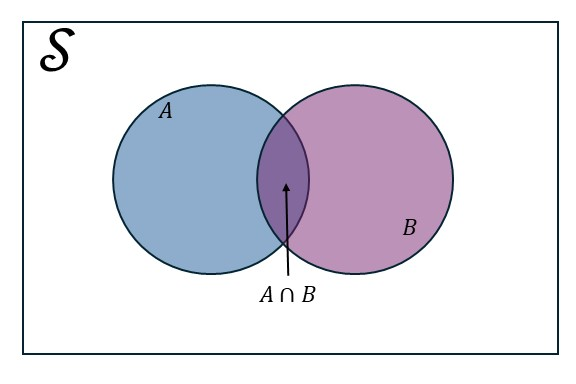
\includegraphics[width = .75\textwidth]{Figures/de_morgans_1_2/Slide1.JPG}
\end{center}
\end{frame}

\begin{frame}{De Morgan's Law}

\begin{center}
\begin{tabular}{cc}
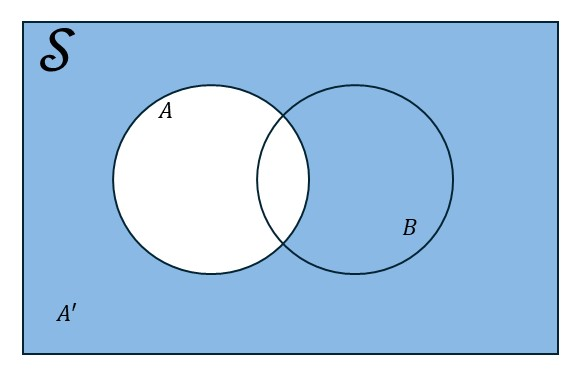
\includegraphics[width = .375\textwidth]{Figures/de_morgans_1_2/Slide2.JPG} &
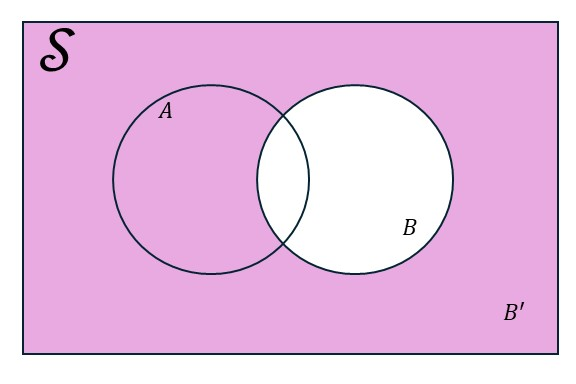
\includegraphics[width = .375\textwidth]{Figures/de_morgans_1_2/Slide3.JPG} \\
\multicolumn{2}{c}{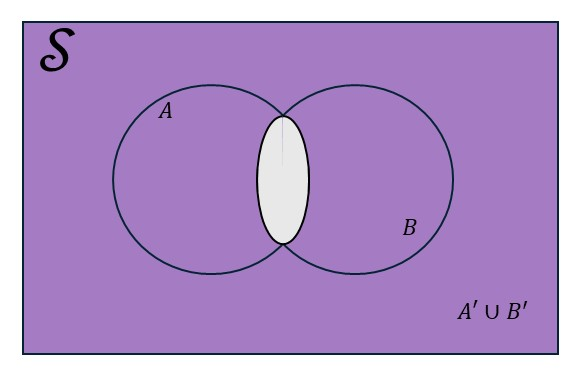
\includegraphics[width = .375\textwidth]{Figures/de_morgans_1_2/Slide4.JPG}}
\end{tabular}
\end{center}
\end{frame}

\begin{frame}{De Morgan's Law}

\textbf{Proof of Part B}

\bigskip

$x \in (A\cup B)'$. Then:
\begin{align*}
x \in (A\cup B)'
\quad iff & \quad x \notin A \cup B\\
\quad iff & \quad x \in A' \quad \mathrm{ and } \quad x \in B'\\
\quad iff & \quad x \in A' \cap B'.\\
\end{align*}

Therefore, $(A\cup B)'=A' \cap B'$
\end{frame}

\begin{frame}{Example 1.1 part 2}
  \begin{block}{Happy Birthmonth!}
    Consider the month of birth for three students selected randomly from the class (call them Alexandria, Braden, and Chen).

    \medskip
    
    Let $A_i$ denote the event that Alexandria is born in month $i$.
    Let $B_i$ denote the event that Braden is born in month $i$.
    Let $C_i$ denote the event that Chen is born in month $i$.

    \medskip
    
    Describe each of the following events in words?
    \begin{enumerate}[a)]
    \item $E_1=A_1 \bigcap B_1 \bigcap C_1$
    \item $E_2=\bigcup_{i=1}^{12} (A_i \bigcap B_i \bigcap C_i)$
    \item $E_3=\bigcup_{i=1}^{12} (A_i \bigcap B_i \bigcap C_i')$
    \end{enumerate}
  \end{block}
\end{frame}

\begin{frame}{Mutually Exclusive}

Two events $A$ and $B$ are said to be \textbf{disjoint} or \textbf{mutually exclusive} if they share no outcomes:
$$
A \cap B = \emptyset.
$$
\end{frame}

\begin{frame}{Example 1.1 part 3}
  \begin{block}{Happy Birthmonth!}
    Consider the month of birth for three students selected randomly from the class (call them Alexandria, Braden, and Chen).

    
    \medskip
    
    Let $A_i$ denote the event that Alexandria is born in month $i$.
    Let $B_i$ denote the event that Braden is born in month $i$.
    Let $C_i$ denote the event that Chen is born in month $i$.

    \medskip
    
    \begin{enumerate}[a)]
    \item Identify two events that are disjoint/mutually exclusive.
    \item Identify two events that are \textit{not} disjoint/mutually exclusive.
    \end{enumerate}
  \end{block}
\end{frame}

\begin{frame}{Set Builder Notation}

  Set builder notation is an easy way to describe events (sets) by characterizing the properties of its outcomes (elements) rather than listing all possible outcomes (elements):
  \[
    \mathcal{S}=\left\{\mbox{type} |  \mbox{restrictions} \right\}.
  \]

  \pause
  
  \begin{block}{Examples}
    \begin{enumerate}
    \item $\mathbb Q = \left\{x \in \mathbb{R} | x=\frac{a}{b} \mbox{ for some } a,b \in \mathbb{Z}, \textcolor{red}{b\neq 0}\right\}$ is the set of rational numbers.
    \item $\mathcal P= \left\{x \in \mathbb{Z} | x=2^c \mbox{ for some } c \in \mathbb{Z}^+ \right\}$ is the set of powers of 2.
    \item $\mathcal S= \left\{(a,b,c) | a,b,c \in \{1,\ldots,12\} \right\}$ is the sample space of the birthday experiment.
    \end{enumerate}
  \end{block}
\end{frame}

\begin{frame}{Example 1.1 part 4}
  \begin{block}{Happy Birthmonth!}
    Consider the events $E_1$, $E_2$, and $E_3$ from part 2.
    \medskip
    
    \begin{enumerate}[a)]
    \item What is the probability of each event?
    \item What do these probabilities mean?
    \end{enumerate}
  \end{block}
\end{frame}

\begin{frame}{Exercise 1.1}

  An unfortunate student has tests in biology, chemistry, and statistics all in one day (a cruel experiment). Thankfully, each test is graded on a pass/fail basis. 
  
  \begin{enumerate}
  \item List all of the outcomes in the sample space.
  \item Write the sample space in set builder notation.
  \item Identify i) two events that are mutually exclusive and ii) two events that are not mutually exclusive.
  \item Let $E_1$ be the event the student passes one test and $E_2$ the event they pass two test. List the outcomes in and describe the event $(E_1 \cup E_2)'$.
  \end{enumerate}
\end{frame}

\begin{frame}
  \begin{center}
    \Large{\textbf{Questions?}}
  \end{center}
\end{frame}

\end{document}
